\section{Mesh motion techniques}
In this section we compare different mesh motion techniques from \ref{sec:meshmotion}. The test will be run using a version of the CSM test discussed earlier. The tests will compare the different techniques by looking at the how the deformation is lifted into the fluid domain. This is done by looking at a plot of the mesh after deformation to see how much cells distort and why. This is done using Paraview.\newline
In these test cases we have the fluid initially at rest and with no inflow on the fluid. A gravitational force is applied to the structure much like the previous CSM test. The only difference is that we now use the full domain from the \ref{sec:HronTurek} . The tests are run as time-dependent with a the backward Euler scheme, leading to a steady state solution. In the first test case the parameters from CSM1 are used, and in the CSM4 the gravitational force has just been increased from 2 to 4. 
\subsection*{Boundary conditions}
The upper, lower and left boundary is set as no slip, that is no velocity in the fluid. On the left boundary there is a do nothing, and zero pressure. 
\subsection*{Quantities for comparison}
The different techniques will be plotted with the minimal value of the Jacobian. The Jacobian is if we remember the determinant of the deformation rate. If the jacobian is zero anywhere in the domain it means that the cells overlap and can cause singularity in the matrices during assembly. \newline
We will also look at the a plot of the deformation in the domain. To visualize the how the different mesh motion techniques work. It is possible to see that if get thin triangles in the computational domain then the mesh motion operator is no good. 

\subsection*{CSM1}
\begin{figure}[H]
\label{fig:fluid_structure}
\caption{CSM1}
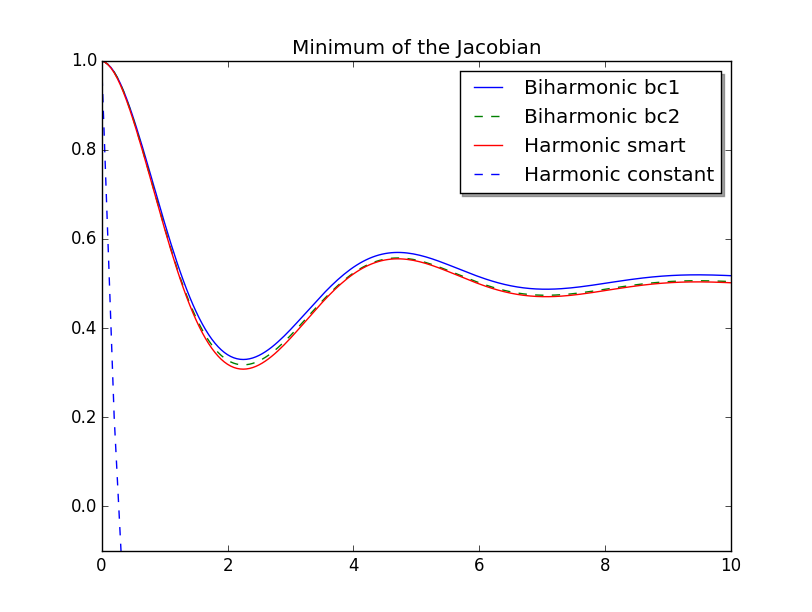
\includegraphics[scale=0.60, trim={0mm 0mm 0mm 0mm},clip]{./Verification_Validation/Mesh_motion_results/CSM1.png}
\end{figure}
